\documentclass[14pt]{extarticle}
% Full article preamble (duplicated, no common file)
\usepackage{fontspec}
\usepackage[a4paper,margin=2.5cm,includefoot]{geometry}
\usepackage{polyglossia}
\usepackage{amsmath}
\usepackage{amssymb}
\usepackage{xcolor}
\usepackage{fancyhdr}
\usepackage{graphicx}
\usepackage{listings}
\usepackage[most]{tcolorbox}
\usepackage{pifont}
\usepackage{enumitem}
\usepackage{titlesec}
\usepackage[bottom]{footmisc}
\usepackage{titling}
\usepackage{minted}
\usepackage{etoolbox}
\usepackage{array}
\usepackage{extsizes}

\newfontfamily\emoji{Segoe UI Emoji}

\pagestyle{fancy}

\setmainlanguage[numerals=western]{arabic}
\setotherlanguage{english}
\newfontfamily\arabicfont[Script=Arabic]{Amiri}
\newfontfamily\arabicfonttt[Script=Arabic]{Courier New}

\lstset{
  language=[Sharp]C,
  numbers=left,
  stepnumber=1,
  numbersep=8pt,
  frame=single,
  basicstyle=\ttfamily\small,
  keywordstyle=\color{blue},
  stringstyle=\color{red},
  commentstyle=\color{green!50!black}
}

\newif\ifdetailed
\ifdefined\setdetailed
  \setdetailed
\fi

\newif\ifwithsols
\ifdefined\setwithsols
  \setwithsols
\fi

% unified tcolorboxes for articles
\tcbset{colback=white, colframe=black, fonttitle=\bfseries, boxrule=0.8pt}
\newtcolorbox{boxDef}[1][]{colback=blue!5!white,colframe=blue!75!black,
  title={{\emoji📘} تعريف\ifx\\#1\\\else ~#1\fi :}}
\newtcolorbox{boxExercise}[1][]{colback=cyan!5!white,colframe=cyan!70!black,
  title={{\emoji🧩} تمرين\ifx\\#1\\\else ~#1\fi :}}
\newtcolorbox{boxExample}[1][]{colback=yellow!5!white,colframe=orange!90!black,
  title={{\emoji📝} مثال\ifx\\#1\\\else ~#1\fi :}}
\newtcolorbox{boxNote}[1][]{colback=gray!10!white,colframe=black,
  title={{\emoji✨} ملاحظة\ifx\\#1\\\else ~#1\fi :}}
\newtcolorbox{boxAttention}[1][]{colback=magenta!10!white,colframe=magenta!80!black,
  title={{\emoji🔔} تنبيه\ifx\\#1\\\else ~#1\fi :}}
\newtcolorbox{boxWarning}[1][]{colback=red!5!white,colframe=red!75!black,
  title={{\emoji⚡} ملاحظة هامة\ifx\\#1\\\else ~#1\fi :}}
\newtcolorbox{boxSolution}[1][]{colback=green!5!white,colframe=green!60!black,
  title={{\emoji✅} حل\ifx\\#1\\\else ~#1\fi :}}
\newtcolorbox{boxSymbol}[1][]{colback=purple!5!white,colframe=purple!70!black,
  title={{\emoji🔣} رمز\ifx\\#1\\\else ~#1\fi :}}

\tcbset{simplecode/.style={ colback=gray!5, colframe=black!50, boxrule=0.4pt, arc=2pt, left=4pt,right=4pt,top=4pt,bottom=4pt}}
\newenvironment{boxCode}{\begin{tcolorbox}[simplecode]}{\end{tcolorbox}}

\newcolumntype{C}[1]{>{\centering\arraybackslash}p{#1}}

% redefine spaces after titles
\makeatletter
\renewcommand{\@maketitle}{%
  \begin{center}
    {\huge \bfseries \@title \par}%
    \vskip 0.2em % space between title and author
    {\large \@author \par}%
    % \vskip 0.2em % space between author and date
    % {\normalsize \@date \par}%
  \end{center}
}
\makeatother

\fancyhf{} % clear default
\fancypagestyle{plain}{
  \fancyhf{}
  \fancyhead[L]{مدرسة التسامح الشاملة}
  % \fancyhead[L]{
\includegraphics[height=1cm]{../../../images/logoTasamoh.png}}
  \fancyhead[R]{الأستاذ محمود اغبارية}
  \fancyfoot[C]{\thepage}
}

\fancyhead[L]{مدرسة التسامح الشاملة}
\fancyhead[R]{الأستاذ محمود اغبارية}
\fancyfoot[C]{\thepage}
% \date{\today}

\setcounter{tocdepth}{3} % only section subsection and subsubsection in TOC


% ----------------------


% \begin{document}

% \maketitle

% % \clearpage  % start TOC on a new page
% % \renewcommand{\contentsname}{جدول المحتويات}
% % \tableofcontents
% % \clearpage

% \part*{part 1} % the * prevents numbering
% \section*{مقدمة}
% \subsection*{مثال رياضي}
% \subsubsection*{مثال فرعي}
% \paragraph*{ paragraph 1}
% \subparagraph*{sub paragraph 1}

% \ifdetailed
% \begin{english}
% \begin{minted}{csharp}
% // C# Example
% \end{minted}
% \end{english}
% \fi

% OLD WAY
% \ifdetailed
% \begin{english}
% \begin{lstlisting}
% // C# Example
% \end{lstlisting}
% \end{english}
% \fi

% % 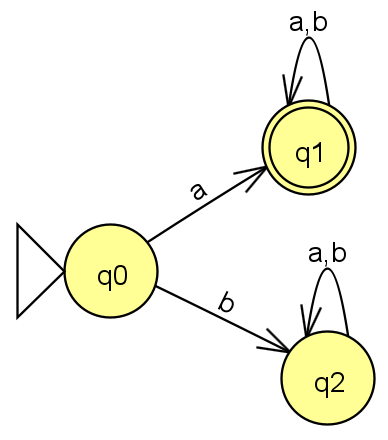
\includegraphics[width=0.2\textwidth]{../../../images/DFAs/ex1_q1.png}



% \vspace{3cm}
% \begin{flushleft}
% أرجو لكم وقتًا ممتعًا.

% الأستاذ محمود اغبارية.
% \end{flushleft}


% \end{document}


\title{ورقة تمرن 6 للصف العاشر 10 \\ جمل شرطية مع عمليات خارجية}

\begin{document}
\maketitle
\thispagestyle{fancy}

\setlist[enumerate]{itemsep=0.8em, topsep=0.5em}

\begin{enumerate}[itemsep=3em]

% -------------------------------------------------------
\item
\begin{enumerate}
\item اكتب عملية خارجيّة تتلقى عددين صحيحين، على العملية أن تعيد حاصل طرح العددين.
\item في البرنامج الرئيسي، استدعِ العمليّة من القسم السابق مع العددين 7 و2.
\item في البرنامج الرئيسي، استقبل عددين صحيحين، واستدعِ العمليّة من قسم (أ) مع العددين المُدخلين.\\
البرنامج يطبع \textenglish{same} إذا كان حاصل طرح العددين يساوي 0، وإلا يطبع \textenglish{different}.
\end{enumerate}

\ifwithsols
\begin{boxSolution}
\begin{english}
\begin{minted}{csharp}
public static int Sub(int a, int b)
{
    return a - b;
}

public static void Main()
{
    Console.WriteLine(Sub(7, 2)); // b)

    // c) read two ints and compare to 0
    int x = int.Parse(Console.ReadLine());
    int y = int.Parse(Console.ReadLine());
    int diff = Sub(x, y);
    if (diff == 0)
        Console.WriteLine("same");
    else
        Console.WriteLine("different");
}
\end{minted}
\end{english}
\end{boxSolution}
\clearpage
\fi

% -------------------------------------------------------
\item
\begin{enumerate}
\item اكتب عملية خارجية تتلقى عددًا ثنائي المنزلة وتعيد حاصل جمع منزلتيه.
\item في البرنامج الرئيسي، استدعِ العمليّة من القسم السابق بحيث تُعيد العملية عددًا أكبر من 15.
\end{enumerate}

\ifwithsols
\begin{boxSolution}
\begin{english}
\begin{minted}{csharp}
public static int SumDigitsTwoDigit(int n)
{
    int tens = n / 10;
    int ones = n % 10;
    return tens + ones;
}

public static void Main()
{
    Console.WriteLine(SumDigitsTwoDigit(89));
}
\end{minted}
\end{english}
\end{boxSolution}
\clearpage
\fi

% -------------------------------------------------------
\item
\begin{enumerate}
\item اكتب عملية خارجية تتلقى عددًا صحيحًا، وتعيد القيمة المطلقة له.\\
\textbf{ملاحظة:} لا تستخدم \textenglish{Math.Abs}.
\item في البرنامج الرئيسي، استقبل عددين صحيحين من المستخدم، واطبع الفرق بينهما بالقيمة المطلقة.\\
عليك استخدام العملية التي كتبتها في البند السابق، لا تستخدم \textenglish{Math.Abs}.
\end{enumerate}

\ifwithsols
\begin{boxSolution}
\begin{english}
\begin{minted}{csharp}
public static int Abs(int x)
{
    if (x < 0)
        return -x;
    else
        return x;
}

public static void Main()
{
    int a = int.Parse(Console.ReadLine());
    int b = int.Parse(Console.ReadLine());
    int diff = a - b;
    Console.WriteLine(Abs(diff));
}
\end{minted}
\end{english}
\end{boxSolution}
\fi

% -------------------------------------------------------
\clearpage
\item
\begin{enumerate}
\item اكتب عملية تتلقى عددين عشريّين، وتعيد حاصل القسمة بينهما.\\
على العملية فحص إذا كان العدد الثاني (المقسوم عليه) يساوي صفرًا؛ في هذه الحالة تطبع العملية رسالة
\textenglish{"ERROR: division by 0"}، وتعيد القيمة $0$.
\item في البرنامج الرئيسي، استدعِ العمليّة من القسم السابق مع الأعداد $3.5$ و $7.0$، واطبع النتيجة.
\item في البرنامج الرئيسي، استدعِ العمليّة من القسم السابق مع الأعداد $0$ و $4$، واطبع النتيجة.
\item في البرنامج الرئيسي، استدعِ العمليّة من القسم السابق مع الأعداد $4$ و $0$، واطبع النتيجة.
\item هل نتيجة الطباعة في الفرعين السابقين متشابهة؟ علّل باختصار.
\end{enumerate}

\ifwithsols
\begin{boxSolution}
\begin{english}
\begin{minted}{csharp}
public static double SafeDiv(double a, double b)
{
    if (b == 0)
    {
        Console.WriteLine("ERROR: division by 0");
        return 0;
    }
    return a / b;
}

public static void Main()
{
    Console.WriteLine(SafeDiv(3.5, 7.0)); // b)
    Console.WriteLine(SafeDiv(0, 4));     // c)
    Console.WriteLine(SafeDiv(4, 0));     // d)
}
\end{minted}
\end{english}
\par
في البندين (ج) و(د) القيمة المطبوعة بالأرقام هي 0 في الحالتين، لكن في (د) تظهر أيضًا رسالة خطأ لأن المقسوم عليه صفر؛ إذًا النتيجة ليست متشابهة تمامًا.
\end{boxSolution}
\fi

% -------------------------------------------------------
\clearpage
\item
في دكّانة أبو السعود توجد خدمة توصيل البضائع إلى الزبائن. تكلفة التوصيل تعتمد على وزن البضاعة، حسب الجدول التالي:

\begin{center}
\renewcommand{\arraystretch}{1.3}
\begin{tabular}{|C{5cm}|C{5cm}|}
\hline
\large{\textbf{وزن البضاعة}} & \large{\textbf{تكلفة التوصيل}} \\[0.3cm] \hline
حتى 1 كغم & 10 شواقل \\ \hline
أكثر من 1 كغم إلى 5 كغم & 20 شاقلا \\ \hline
أكثر من 5 كغم & 30 شاقلا \\ \hline
\end{tabular}
\end{center}

\begin{enumerate}
\item اكتب عملية خارجية تستقبل وزن البضاعة (كغم)، وتعيد تكلفة التوصيل (بالشواقل) حسب الجدول أعلاه.
\item في البرنامج الرئيسي، استدعِ العملية من القسم السابق مع الوزن $3.4$ كغم، واطبع تكلفة التوصيل.
\item في البرنامج الرئيسي، استدعِ العملية من القسم السابق مع وزن من اختيارك بحيث تكون التكلفة 10 شواقل.
\item في البرنامج الرئيسي، استقبل من المستخدم وزن البضاعة، واستدعِ العمليّة من القسم السابق، واطبع تكلفة التوصيل.
\end{enumerate}

\ifwithsols
\begin{boxSolution}
\begin{english}
\begin{minted}{csharp}
public static int DeliveryCost(double weightKg)
{
    if (weightKg <= 1.0)
        return 10;
    else if (weightKg <= 5.0)
        return 20;
    else
        return 30;
}

public static void Main()
{
    Console.WriteLine(DeliveryCost(3.4)); // b)
    Console.WriteLine(DeliveryCost(0.75)); // c) -> 10

    double w = double.Parse(Console.ReadLine());
    Console.WriteLine(DeliveryCost(w)); // d)
}
\end{minted}
\end{english}
\end{boxSolution}
\fi

% -------------------------------------------------------
\clearpage
\item
في معهد الحاسوب، لقبول الطالب في دورة البرمجة يجب أن يتحقق \textbf{على الأقل واحد} من الشرطين التاليين:
\begin{itemize}
  \item أن يكون عمره 18 سنة فما فوق.
  \item أن يكون قد أنهى دورة سابقة في البرمجة.
\end{itemize}

\begin{enumerate}
\item اكتب عملية خارجية باسم \textenglish{IsAccepted} تتلقى:
\begin{itemize}
  \item عمر الطالب (عدد صحيح).
  \item وحالة إنهائه لدورة سابقة (بارامتر \textenglish{bool}: \textenglish{true} إذا أنهى دورة، و\textenglish{false} إذا لم ينهِ).
\end{itemize}
على العملية أن تعيد \textenglish{true} إذا تحقق أحد الشرطين أعلاه، وإلا تعيد \textenglish{false}.
\item في البرنامج الرئيسي، استدعِ العمليّة من القسم السابق مع عمر 20 سنة وحالة إنهاء دورة سابقة \textenglish{false}، واطبع الناتج.
\item في البرنامج الرئيسي، استدعِ العمليّة من القسم السابق مع عمر وحالة إنهاء دورة سابقة من اختيارك بحيث ترجع العملية \textenglish{false}.
\item في البرنامج الرئيسي استقبل عددين صحيحين:
  \begin{itemize}
    \item الأول: عمر الطالب.
    \item الثاني: حالة إنهائه لدورة سابقة (1 إذا أنهى الدورة، و0 إذا لم ينهِ).
  \end{itemize}
واستدعِ العمليّة من القسم الأول مع القيم المناسبة حسب ما أدخله المستخدم، واطبع
    \begin{itemize}
      \item \textenglish{Accepted} إذا تحقق أحد الشرطين أعلاه وكان مقبولًا.
      \item \textenglish{Rejected} خلاف ذلك.
    \end{itemize}
\end{enumerate}

\ifwithsols
\begin{boxSolution}
\begin{english}
\begin{minted}{csharp}
public static bool IsAccepted(int age, bool finishedCourse)
{
    if(age >= 18 || finishedCourse)
        return true;
    else
        return false;
}

public static void Main()
{
    // b)
    Console.WriteLine(IsAccepted(20, false));

    // c)
    Console.WriteLine(IsAccepted(17, false));

    // d)
    int age = int.Parse(Console.ReadLine());
    int finished = int.Parse(Console.ReadLine()); // 1 or 0
    bool finishedCourse = (finished == 1);

    if (IsAccepted(age, finishedCourse))
        Console.WriteLine("Accepted");
    else
        Console.WriteLine("Rejected");
}
\end{minted}
\end{english}
\end{boxSolution}
\fi


% -------------------------------------------------------
\clearpage
\item
أمامك مقطع الكود التالي:

\begin{boxCode}
\begin{english}
\begin{minted}{csharp}
public static int DoSomething(int n, int d)
{
    return n * 10 + d;
}

public static void Main()
{
    int d1 = int.Parse(Console.ReadLine());
    int d2 = int.Parse(Console.ReadLine());
    int d3 = int.Parse(Console.ReadLine());
    int d4 = int.Parse(Console.ReadLine());
    int result = DoSomething(d1, d2);
    result = DoSomething(result, d3);
    result = DoSomething(result, d4);
    Console.WriteLine(result);
}
\end{minted}
\end{english}
\end{boxCode}

\begin{enumerate}
\item أكمل الجدول التالي بكتابة الناتج الذي يطبعه البرنامج في كل حالة:

\begin{center}
\renewcommand{\arraystretch}{1.3}
\begin{tabular}{|C{1cm}|C{1cm}|C{1cm}|C{1cm}|C{5cm}|}
\hline
\textbf{$d_1$} & \textbf{$d_2$} & \textbf{$d_3$} & \textbf{$d_4$} & \textbf{الناتج المطبوع} \\ \hline
3 & 1 & 4 & 2 & \\ \hline
5 & 0 & 7 & 8 & \\ \hline
9 & 9 & 0 & 1 & \\ \hline
2 & 3 & 0 & 4 & \\ \hline
0 & 0 & 2 & 7 & \\ \hline
\end{tabular}
\end{center}

\item ما هي وظيفة البرنامج؟ (صفها بسطر واحد)

\item لكل واحد من المخرجات التالية، ما هي المدخلات التي يجب إدخالها للحصول عليه؟

\begin{center}
\renewcommand{\arraystretch}{1.3}
\begin{tabular}{|C{3cm}|C{2cm}|C{2cm}|C{2cm}|C{2cm}|}
\hline
\textbf{الناتج المطبوع} & \textbf{$d_1$} & \textbf{$d_2$} & \textbf{$d_3$} & \textbf{$d_4$} \\ \hline
1235 &  &  &  & \\ \hline
3210 &  &  &  & \\ \hline
798 &  &  &  & \\ \hline
90 &  &  &  & \\ \hline
\end{tabular}
\end{center}
\end{enumerate}

\ifwithsols
\begin{boxSolution}
\begin{center}
\renewcommand{\arraystretch}{1.3}
\begin{tabular}{|C{1cm}|C{1cm}|C{1cm}|C{1cm}|C{5cm}|}
\hline
\textbf{$d_1$} & \textbf{$d_2$} & \textbf{$d_3$} & \textbf{$d_4$} & \textbf{الناتج المطبوع} \\ \hline
3 & 1 & 4 & 2 & 3142 \\ \hline
5 & 0 & 7 & 8 & 5078 \\ \hline
9 & 9 & 0 & 1 & 9901 \\ \hline
2 & 3 & 0 & 4 & 2304 \\ \hline
0 & 0 & 2 & 7 & 27 \\ \hline
\end{tabular}
\end{center}

وظيفة البرنامج: تكوين عدد من أربع خانات من المدخلات بنفس الترتيب.

\begin{center}
\renewcommand{\arraystretch}{1.3}
\begin{tabular}{|C{3cm}|C{2cm}|C{2cm}|C{2cm}|C{2cm}|}
\hline
\textbf{الناتج المطبوع} & \textbf{$d_1$} & \textbf{$d_2$} & \textbf{$d_3$} & \textbf{$d_4$} \\ \hline
1235 & 1 & 2 & 3 & 5 \\ \hline
3210 & 3 & 2 & 1 & 0 \\ \hline
798 & 0 & 7 & 9 & 8 \\ \hline
90 & 0 & 0 & 9 & 0 \\ \hline
\end{tabular}
\end{center}
\end{boxSolution}
\fi

\end{enumerate}
\end{document}
